\large \subsection*{Tuyển tập các dạng bài hay - lạ - khó}

%Câu 1
\begin{vd}
	[Đề HSG cấp cụm Hoài Đức - Hà Đông 2022-2023] Một vật có khối lượng $m = 2\mathrm{kg}$, chuyển động thẳng trên sàn ngang dưới tác dụng của lực $\vec{F}_{\mathrm{k}}$ như hình bên dưới. Hệ số ma sát trượt giữa vật và bề mặt tiếp xúc $\mu = 0,3$, lấy $g = 10\mathrm{m/s^2}$.
	\begin{enumerate}
		\item Cho $\alpha = 30^\circ$, $F_{\mathrm{k}} = 8\mathrm{N}$, tính gia tốc chuyển động của vật và quãng đường vật đi được sau $5\mathrm{s}$ chuyển động.
		\item Tìm giá trị nhỏ nhất của lực $\vec{F}_{\mathrm{k}}$ để làm cho vật chuyển động trên bề mặt tiếp xúc.
	\end{enumerate}
\end{vd}

%Câu 2
\begin{vd}
	Một vật có khối lượng $m = 5\mathrm{kg}$ chuyển động trên sàn nằm ngang dưới tác dụng của một lực kéo $\vec{F}$ hợp với hướng chuyển động một góc $\alpha$ như hình bên dưới. Hệ số ma sát trượt giữa vật và sàn là $\mu = 0,2$. Thay đổi góc $\alpha$ để lực kéo là nhỏ nhất để vật chuyển động thẳng đều, khi đó $\alpha$ có giá trị là?
\end{vd}

%Câu 3
\begin{vd}
	Một vật có khối lượng $4\mathrm{kg}$ được kéo trên mặt sàn nằm ngang bởi lực $F$ hợp với phương ngang góc $\alpha$ như hình bên dưới. Hệ số ma sát trượt giữa vật và sàn là $\mu = 0,3$. Bỏ qua lực cản không khí. Lấy $g = 10\mathrm{m/s^2}$.
	\begin{enumerate}
		\item Cho $\alpha = 30^\circ$ và $F = 15\mathrm{N}$. Tính gia tốc của vật.
		\item Thay đổi góc $\alpha$, tìm độ lớn lực $F$ nhỏ nhất để vật trượt nhanh dần đều trên mặt sàn với gia tốc bằng $0,5\mathrm{m/s^2}$.
	\end{enumerate}
\end{vd}

\begin{center}
	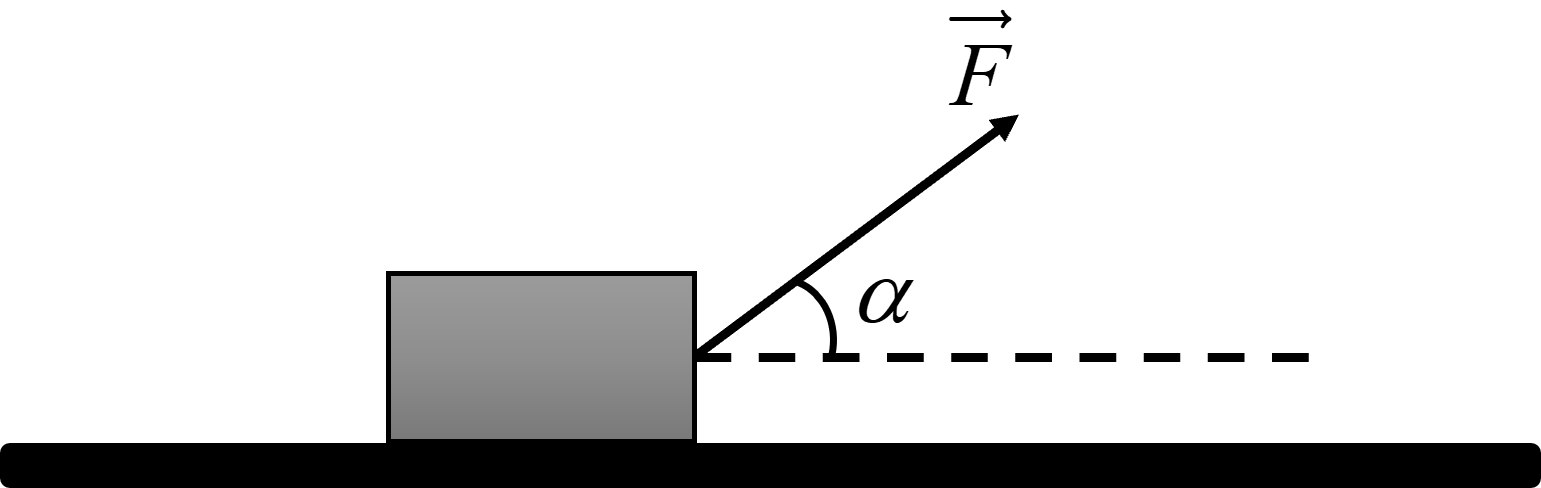
\includegraphics[scale=0.6]{img/H1.png}
\end{center}

%Câu 4
\begin{vd}
	Vật khối lượng $m$ được kéo đi lên trên mặt phẳng nghiêng với lực $\vec{F}$, $\vec{F}$ hợp với mặt phẳng nghiêng góc $\beta$. Mặt phẳng nghiêng góc $\alpha$ so với mặt phẳng ngang. Hệ số ma sát trượt giữa vật và mặt phẳng nghiêng là $\mu$.
	\begin{center}
		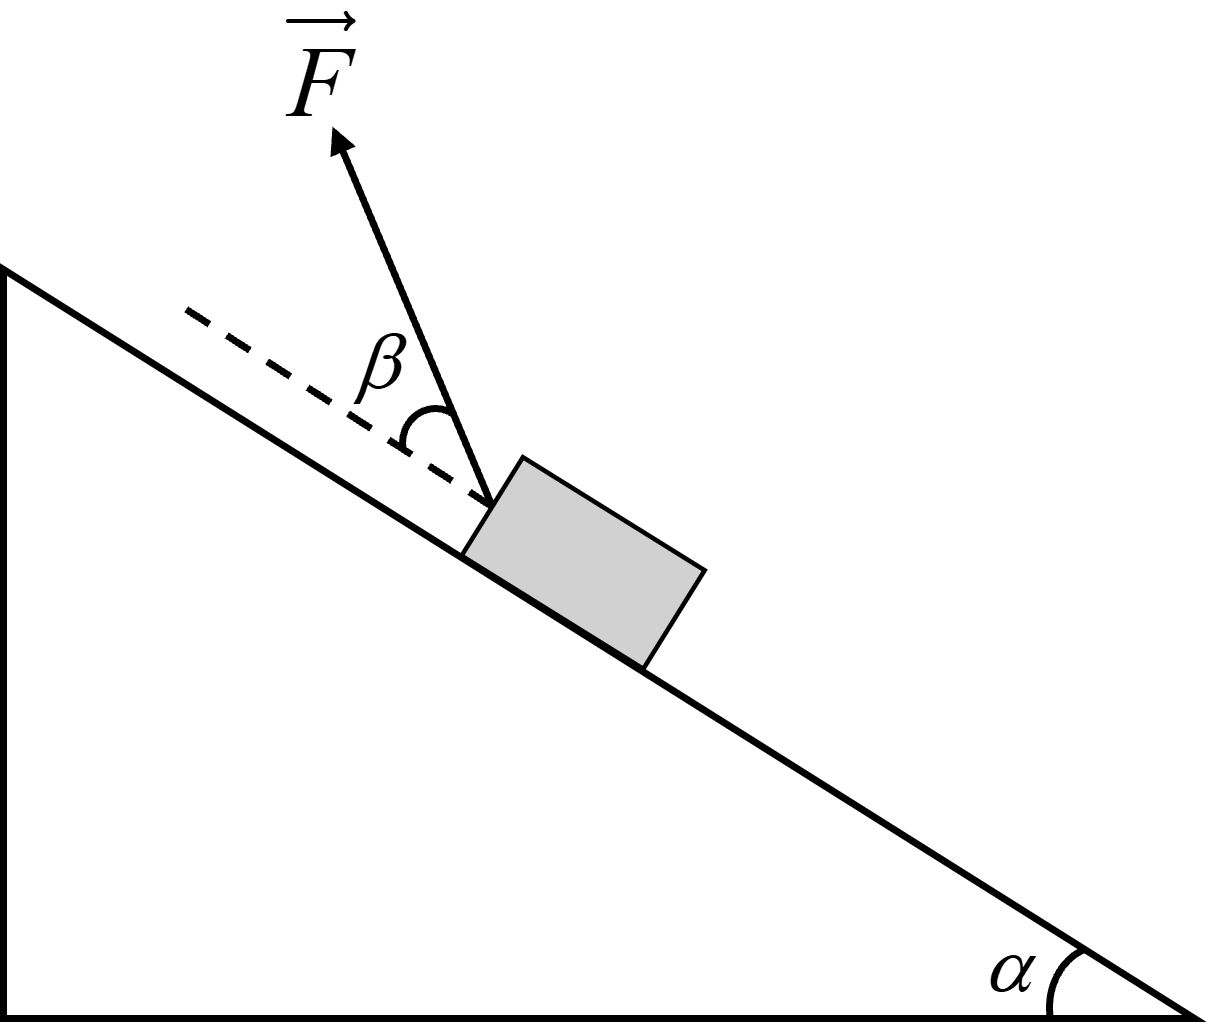
\includegraphics[scale=0.6]{img/C4.png}
	\end{center}
	\begin{enumerate}
		\item Tìm biểu thức tính $F$ khi vật đi lên đều theo mặt phẳng nghiêng.
		\item Với $m = 5\mathrm{kg}$, $\alpha = 45^\circ$, $\mu = 0,5$, lấy $g = 10\mathrm{m/s^2}$. Xét vật đi lên đều, tìm $\beta$ để $F$ nhỏ nhất, tìm giá trị lực $F$ nhỏ nhất đó.
	\end{enumerate}

\end{vd}

\begin{vd}
	Một vật có trọng lượng $P = 100\mathrm{N}$ được giữ đứng yên trên mặt phẳng nghiêng góc $\alpha$ bằng lực $F$ có phương nằm ngang như hình vẽ. Biết $\tan\alpha = 0,5$ và hệ số ma sát trượt $\mu = 0,2$. Lấy $g = 10\mathrm{m/s^2}$.
	\begin{center}
		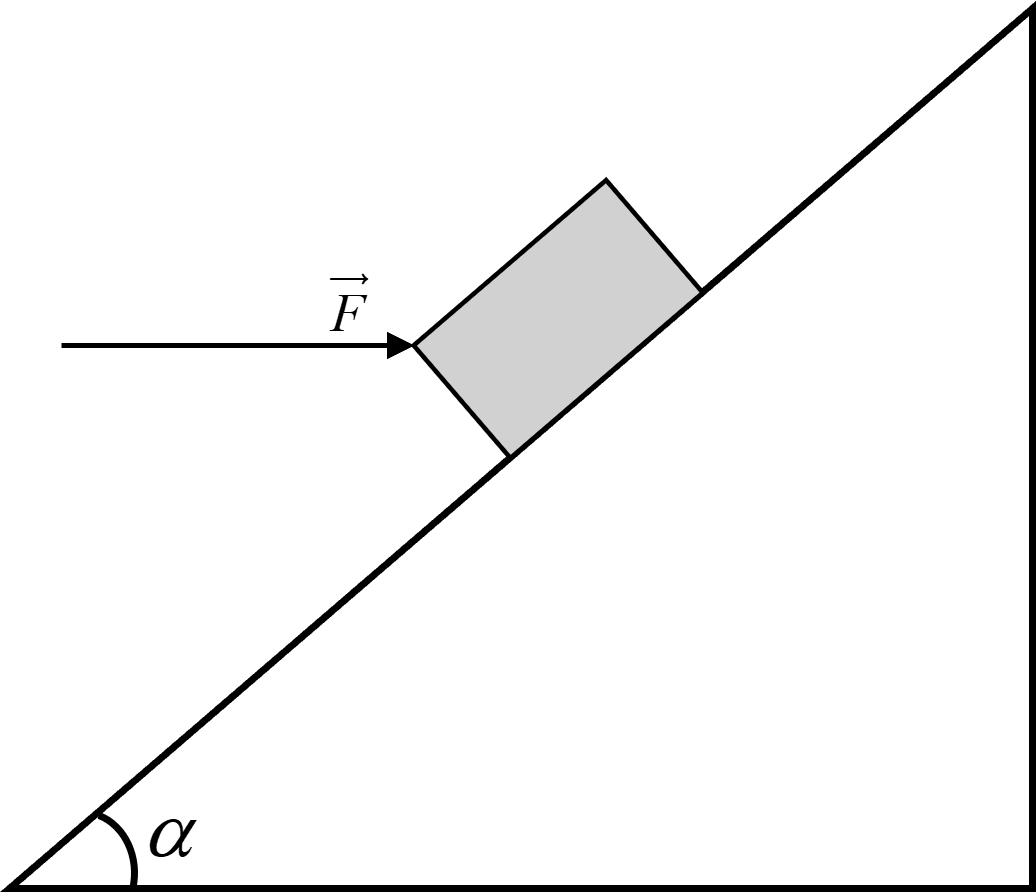
\includegraphics[scale=0.6]{img/C5.png}
	\end{center}
	\begin{enumerate}
		\item Tính giá trị lực $F$ lớn nhất.
		\item Tính giá trị lực $F$ nhỏ nhất.
	\end{enumerate}

\end{vd}

\begin{vd}
	Một hộp chứa cát ban đầu đứng yên, được kéo trên sàn ngang bằng một sợi dây chịu được sức căng cực đại là $T_{\max}$. Hệ số ma sát giữa hộp và sàn là $\mu$. Góc hợp bởi dây và phương ngang là $\alpha$.
	\begin{enumerate}
		\item Tính gia tốc của hộp biết lực kéo tác dụng vào dây là $F$.
		\item Để kéo được lượng cát lớn nhất thì góc $\alpha$ phải là bao nhiêu? Áp dụng bằng số: $T_{\max} = 500\mathrm{N}$, $\mu = 0,25$.
		\item Trọng lượng tổng cộng của hộp cát ứng với góc $\alpha$ tính được ở câu b là bao nhiêu?
	\end{enumerate}
\end{vd}

\begin{vd}
	[Đề HSG cụm Chương Mỹ-Thanh Oai 2022-2023] Một diêm dân (người làm muối) đang thu gom muối trên ruộng có kéo một xe trượt là một thùng gỗ, ở đầu có buộc một sợi dây. Lực kéo của người tác dụng lên dây có độ lớn không đổi là $100\mathrm{N}$. Cho hệ số ma sát trượt giữa thùng gỗ với cát là $0,35$. Lấy $g = 10\mathrm{m/s^2}$, coi khối lượng của thùng gỗ không đáng kể.
	\begin{enumerate}
		\item Khi kéo lượng muối trong thùng là $m = 15\mathrm{kg}$, dây kéo được người đó quấn quanh bụng, biết khoảng cách từ chỗ bụng quấn dây đến mặt đất là $d = 70\mathrm{cm}$, khoảng cách từ bàn chân người đó đến hộp là $l = 1,4\mathrm{m}$. Tìm công kéo thùng muối mà người đó đã thực hiện được sau $2\mathrm{s}$ kể từ khi thùng muối bắt đầu chuyển động?
		\item Hỏi góc giữa dây kéo và phương ngang bằng bao nhiêu để người đó kéo được lượng muối là lớn nhất? Tìm khối lượng muối lớn nhất người đó có thể kéo được?
	\end{enumerate}
\end{vd}

\begin{vd}
	[Đề HSG cấp trường HĐA 2021-2022] Vật $m_1 = 0,2\mathrm{kg}$, $m_2 = 0,1\mathrm{kg}$ được nối với nhau bằng một sợi chỉ mảnh không khối lượng, không co giãn vắt qua ròng rọc. Các vật đó nằm trên các mặt phẳng nghiêng có một góc $\alpha = 15^\circ$, $\beta = 6^\circ$ so với phương nằm ngang (hình vẽ). Trước khi chuyển động các khối lượng đó nằm trên cùng một độ cao. Biết rằng hệ số ma sát trượt giữa các mặt phẳng nghiêng và các khối lượng là $\mu = 0,1$. Bỏ qua khối lượng ròng rọc, ma sát ở trục ròng rọc. Hãy xác định sự chênh lệch về độ cao $h$ của các vật $m_1$ và $m_2$ sau thời gian $t = 3$ giây kể từ khi thả cho chúng chuyển động.
	\begin{center}
		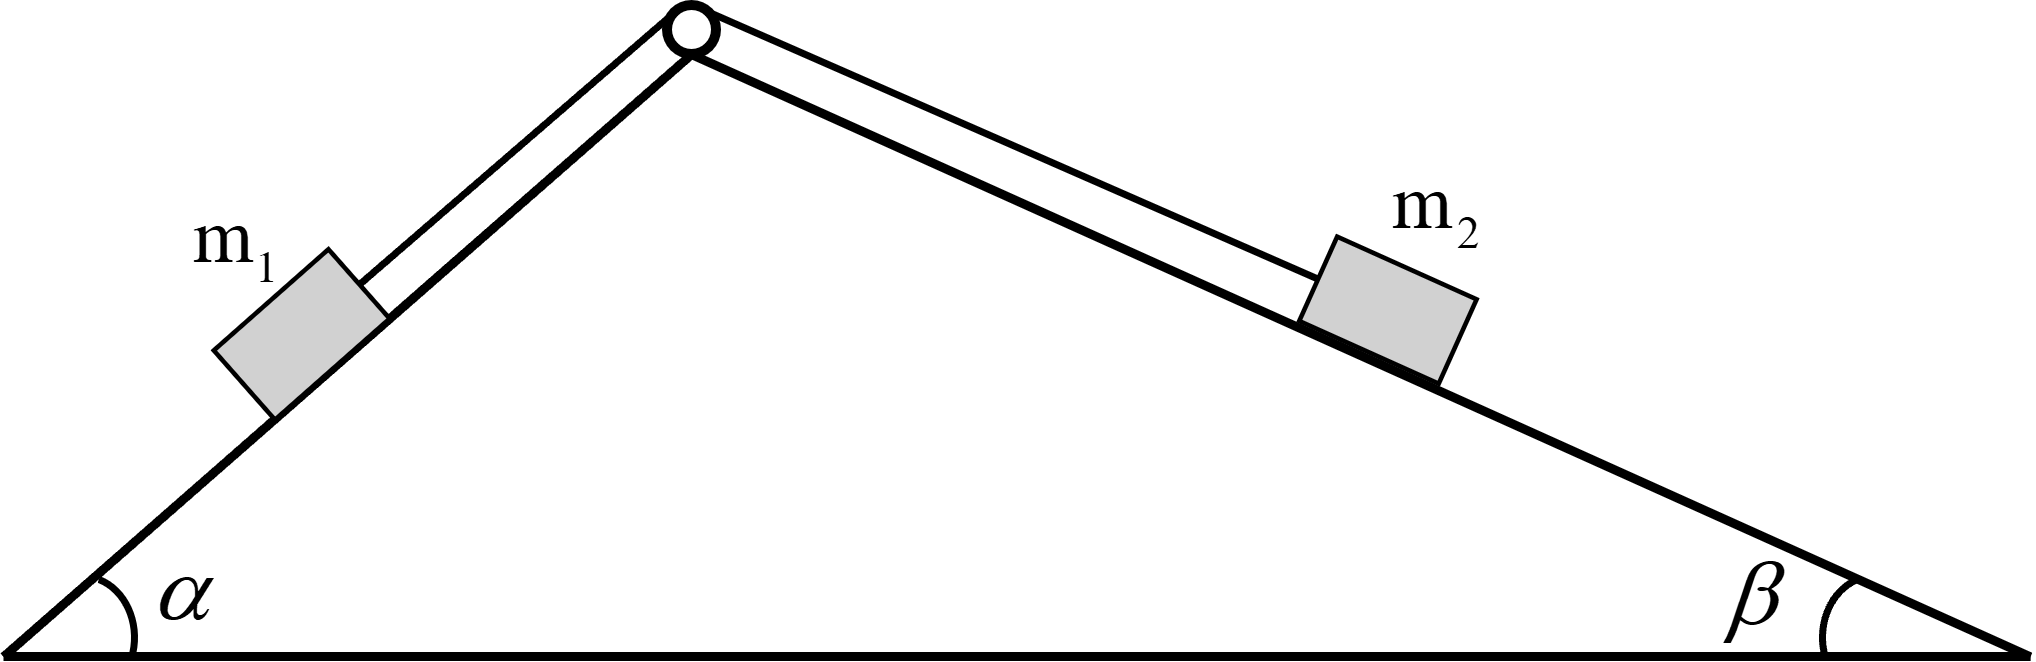
\includegraphics[scale=0.6]{img/C7.png}
	\end{center}
\end{vd}

\begin{vd}
	[Đề HSG cấp cụm Hoài Đức - Hà Đông 2022-2023] Cho cơ hệ như hình vẽ. Biết $\alpha = 30^\circ$, $m_1 = 3\mathrm{kg}$, $m_2 = 2\mathrm{kg}$, một nêm $M = 2\mathrm{kg}$, ma sát giữa $m_2$ và $M$ là không đáng kể. Bỏ qua khối lượng dây nối và ròng rọc, dây không dãn, lấy $g = 10\mathrm{m/s^2}$.
	\begin{center}
		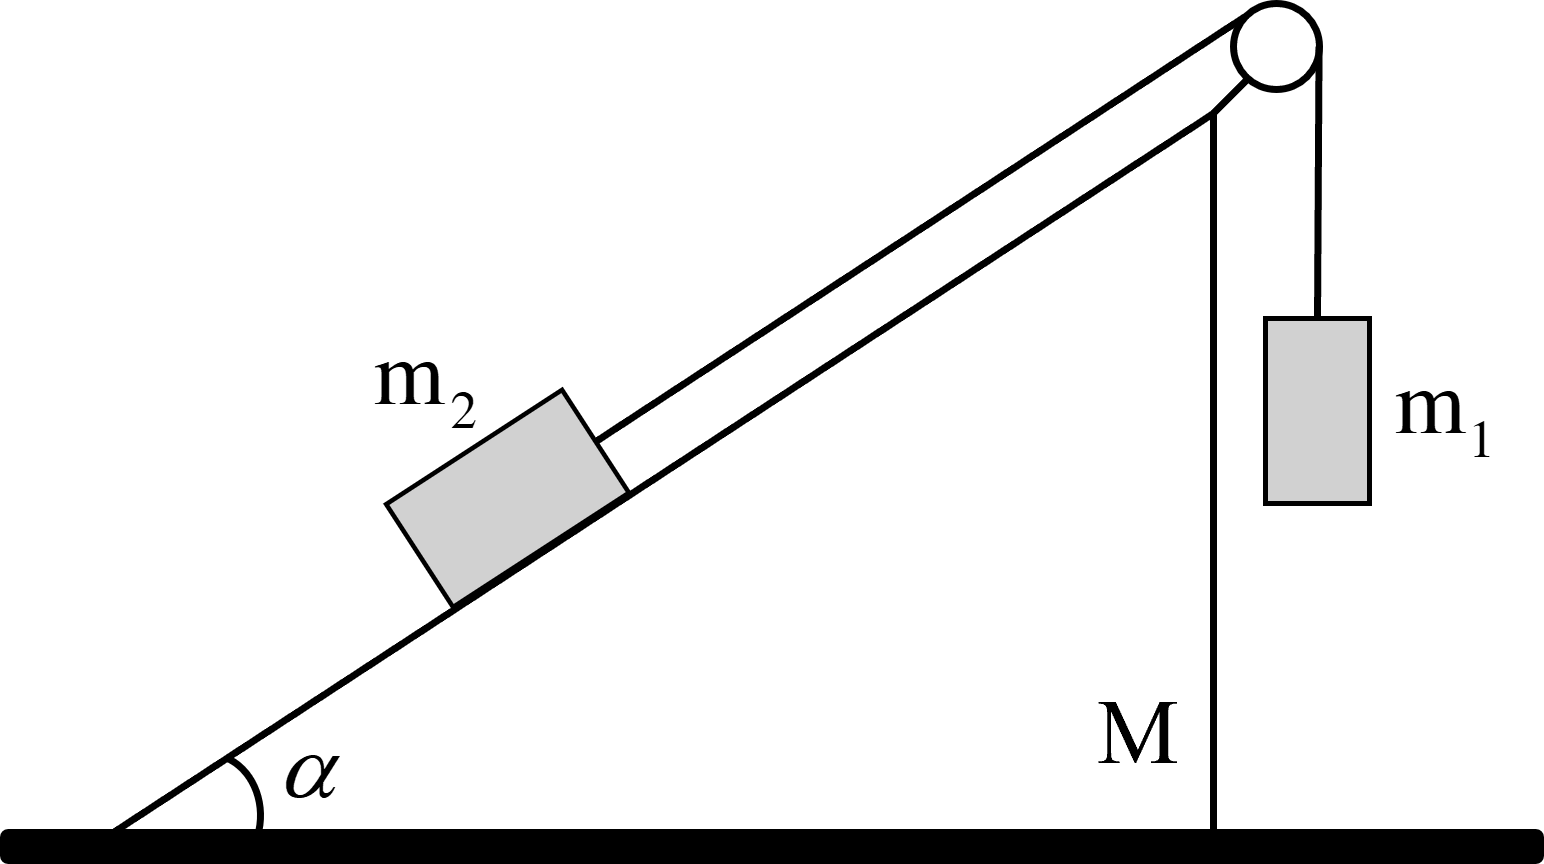
\includegraphics[scale=0.6]{img/C8.png}
	\end{center}
	\begin{enumerate}
		\item $M$ đứng yên, tìm gia tốc của các vật $m_1$, $m_2$ và áp lực của dây lên ròng rọc.
		\item Tìm điều kiện của hệ số ma sát giữa $M$ và mặt sàn nằm ngang để $M$ không bị trượt trên sàn.
	\end{enumerate}
\end{vd}

\begin{vd}
	Hai vật A và B có khối lượng lần lượt là $m_1 = 3\mathrm{kg}$ và $m_2 = 2\mathrm{kg}$ nối với nhau bằng một sợi dây vắt qua ròng rọc gắn ở đỉnh mặt phẳng nghiêng nhẵn cố định, đủ dài với góc nghiêng $\alpha = 30^\circ$ như hình vẽ. Ban đầu A được giữ ở vị trí ngang với B, thả cho hai vật chuyển động. Lấy $g = 10\mathrm{m/s^2}$.
	\begin{center}
		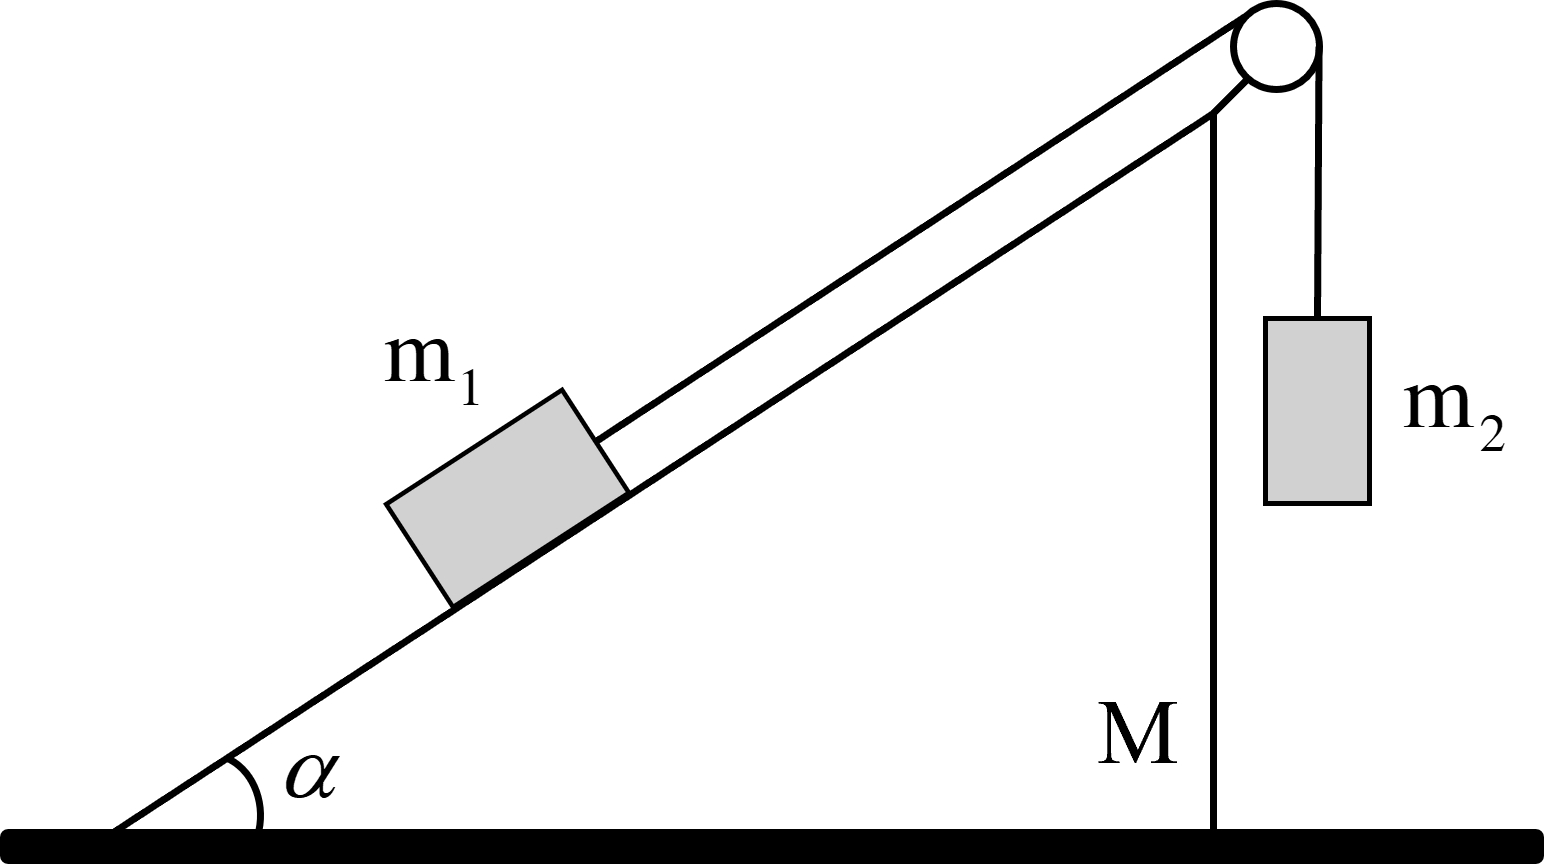
\includegraphics[scale=0.6]{img/C9.png}
	\end{center}
	\begin{enumerate}
		\item Hai vật chuyển động theo chiều nào.
		\item Tính lực căng của dây và lực nén lên trục ròng rọc. Bỏ qua ma sát, khối lượng của ròng rọc và dây.
		\item Tại thời điểm vật nọ thấp hơn vật kia một đoạn bằng $0,75\mathrm{m}$ thì dây nối hai vật bị đứt. Tính hiệu độ cao giữa hai vật sau khi dây đứt $0,8\mathrm{s}$. Biết B có độ cao đủ lớn.
	\end{enumerate}
\end{vd}

\begin{vd}
	[Đề HSG cấp trường HĐA 2022-2023] 
	Vật A bắt đầu trượt từ đầu tấm ván B nằm ngang (như hình vẽ). Vận tốc ban đầu của A là $3\mathrm{m/s}$, của B là $0\mathrm{m/s}$. Hệ số ma sát giữa A và B là $0,25$. Mặt sàn là nhẵn. Chiều dài của ván B là $1,6\mathrm{m}$. Vật A có khối lượng $m_1 = 200\mathrm{g}$, vật B có khối lượng $m_2 = 1\mathrm{kg}$. Hỏi A có trượt hết tấm ván B không? Nếu không, hãy tính quãng đường A đi được trên tấm ván B và cho biết hệ sau đó chuyển động như thế nào với vận tốc bao nhiêu? Lấy $g = 10\mathrm{m/s^2}$.
	\begin{center}
		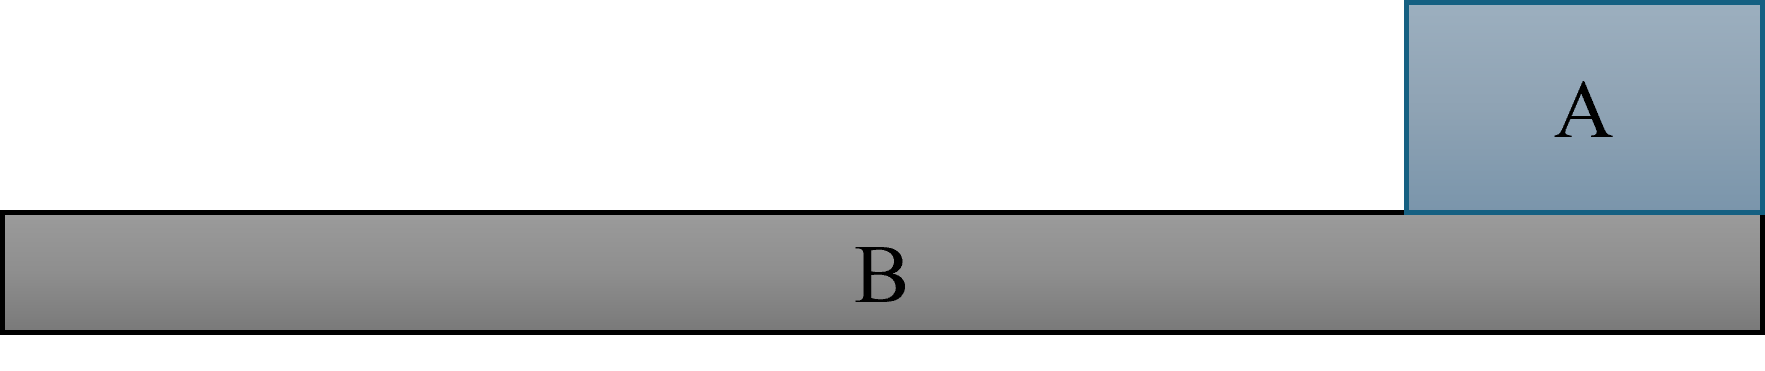
\includegraphics[scale=0.6]{img/7.png}
	\end{center}
\end{vd}

\begin{vd}
	Hai vật cùng khối lượng $m = 1\mathrm{kg}$ được nối với nhau bằng sợi dây không dãn và khối lượng không đáng kể. Một trong hai vật chịu tác dụng của lực kéo hợp với phương ngang góc $\alpha = 30^\circ$. Hai vật có thể trượt trên mặt bàn nằm ngang. Hệ số ma sát giữa vật và bàn là $0,268$. Biết rằng dây chỉ chịu được lực căng lớn nhất là $10\mathrm{N}$. Tính lực kéo lớn nhất để dây không đứt. Lấy $\sqrt{3} = 1,732$, $g = 10\mathrm{m/s^2}$.
	\begin{center}
		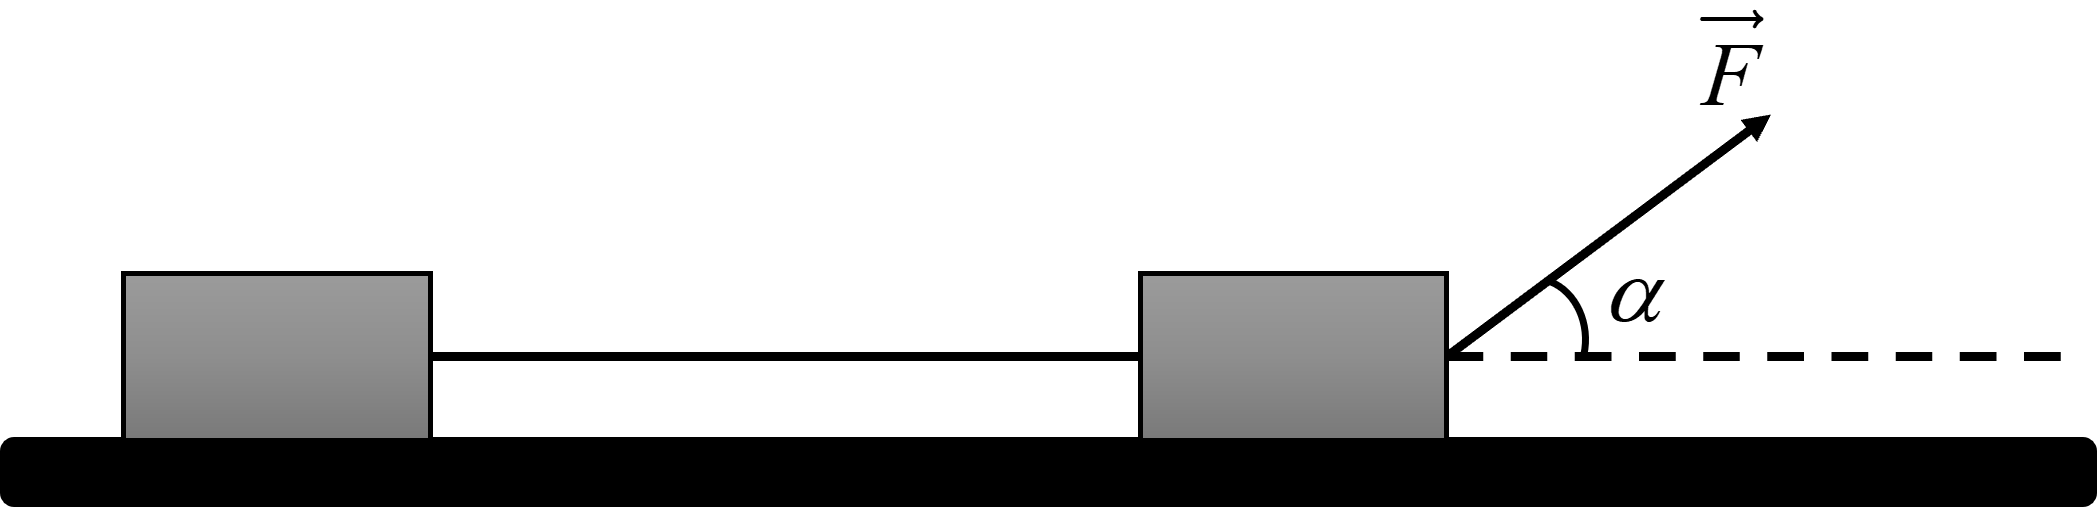
\includegraphics[scale=0.6]{img/8.png}
	\end{center}
\end{vd}

\newpage
\begin{vd}%[Nguyễn Tấn Linh]%[2H2B1-1]
%	[Đề minh họa BDG 2019-1020] 
	Hình bên là cấu trúc tinh thể muối ăn (NaCl). Các ion $Na^{+}$ và $Cl^{-}$ sắp xếp xen kẽ cách đều nhau theo ba hướng vuông góc với nhau. Biết muối ăn có khối lượng mol là $58,5 \ g/mol$ và khối lượng riêng là $2,2 \ g/cm^{3}$. Khoảng cách giũa hai ion $Na^{+}$ gần nhất trong tinh thể muối ăn là bao nhiêu? Lấy $N_A = 6,02.10^{23} \ mol^{-1}$.
	\begin{center}
		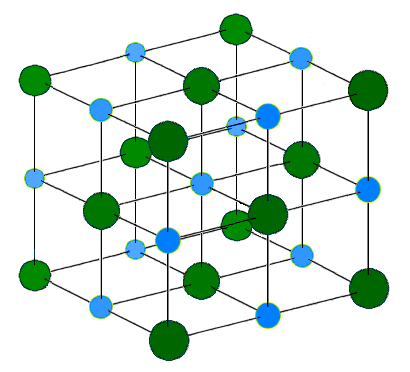
\includegraphics[scale=1.2]{img/Sodium_chloride_crystal.png}
	\end{center}
	\loigiai{
		\begin{phantich}
			Dựa vào mô hình phân tử muối ăn, ta thấy khoảng cách giữa hai ion $Na^{+}$ gần nhất là $d = a\sqrt{2}$, với $a$ là độ dài cạnh của ô cơ sở.
		\end{phantich}
		Nếu không phân biệt ion, thí các ion sắp xếp cách đều nhau.\\
		Thể tích không gian chiếm chỗ của mỗi ion là:  ${V_0} = \dfrac{{{V_m}}}{{2{N_A}}} = \dfrac{M}{{2\rho {N_A}}}$\\
		Mà ${V_0} = {a^3} \to a = \sqrt[3]{{{V_0}}}$\\
		Khoảng cách giữa hai ion gần nhất là $d = a\sqrt 2  = \sqrt[3]{{\dfrac{M}{{2\rho {N_A}}}}}.\sqrt 2  = 3,{97.10^{ - 8}} \ cm$.
	}
\end{vd}

\begin{vd}
	Hình bên là cấu trúc tinh thể caesium clorua (CsCl), ion $Cl^-$ nằm ở tâm của khối lập phương và ion $Cs^+$ nằm ở tám đỉnh của khối lập phương. Biết khối lượng mol của caesium clorua là $168 \ g/mol$, khoảng cách gần nhất giữa hai ion $Cl^-$ là $4.10^{-10} \ m$. Khối lượng riêng của caesium clorua là bao nhiêu? Lấy $N_A = 6,02.10^{23} \ mol^{-1}$.
	\begin{center}
		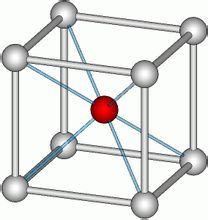
\includegraphics[scale=0.4]{img/8412619e887615d09147c0aadc784128.jpg}
	\end{center}
	\loigiai{
		\begin{phantich}
			Khoảng cách gần nhất giữa hai ion $Cl^-$ là độ dài cạnh $a$ của hình lập phương.\\
			Vì các ion $Cs^+$ sắp xếp đều nhau nên mỗi ion chiếm không gian bằng khối lập phương.
		\end{phantich}
		Thể tích mol là ${{V}_{m}}={{V}_{0}}.{{N}_{A}}={{a}^{3}}.{{N}_{A}}$\\\\
		Khối lượng riêng của $CsCl$ là $\rho =\dfrac{M}{{{V}_{m}}}=\dfrac{M}{{{a}^{3}}.{{N}_{A}}}=4,36 \ g/c{{m}^{3}}$
	}
\end{vd}

\begin{vd}
	Biết khí quyển Trái Đất có độ dày nhỏ hơn nhiều so với bán kính $R = 6,4.10^6 \ m$ của Trái Đất, khối lượng mol trung bình là $M = 29 \ g/mol$. Lấy $N_A = 6,02.10^{23} \ mol^{-1}$, áp suất khí quyển ở mặt đất là $p_0 = 10^5 \ Pa$, và gia tốc rơi tự do là $g = 10 \ m/s^2$. Tổng số phân tử trong khí quyển Trái Đất ước lượng là bao nhiêu?
	\loigiai{
		\begin{phantich}
			Áp suất khí quyển là do trọng lực tác dụng lên bề mặt Trái Đất gây ra.\\
			Từ các số liệu đề cho, ta tính được khối lượng khí quyển rồi suy ra được số phân tử.
		\end{phantich}
		Diện tích bề mặt Trái Đất là $S=4\pi {{R}^{2}}$\\
		Khối lượng khí trong khí quyển: ${{p}_{o}}=\dfrac{mg}{S}\to m=\dfrac{4{{p}_{0}}\pi {{R}^{2}}}{g}$\\\\
		Số phân tử trong khí quyển là $N=n{{N}_{A}}=\dfrac{m}{M}{{N}_{A}}=\dfrac{4{{p}_{0}}\pi {{R}^{2}}}{Mg}{{N}_{A}}$\\\\
		Thay số ta được $N = 10^{44}$ phân tử.
	}
	
\end{vd}

\begin{vd}
	Hàm số bậc ba $y = ax^{3} + bx^{2} + cx +d$ $(a \neq 0)$ thỏa mãn các điều kiện sau
\end{vd}